\documentclass{beamer}
\mode<presentation>
{ \usetheme{boxes} }

\usepackage{times}
\usepackage{graphicx}
\usepackage[backend=bibtex]{biblatex}
\usepackage{verbatim}
% \addbibresourse{an_introduction_to_dogen.bib}

\title{Using Watertight Polygon Meshes for Neuronal Morphology Representation}
\author{
  \texorpdfstring
      {\href{mailto:marco.craveiro@gmail.com}{Marco Craveiro}}
      {Marco Craveiro}
}
\date{\today}

\AtBeginSection[]
{
  \begin{frame}<beamer>
    \frametitle{Outline}
    \tableofcontents[currentsection]
  \end{frame}
}

\bibliography{watertight}

\begin{document}

\begin{frame}
\titlepage
\end{frame}

\begin{frame}
\frametitle{Outline}
\begin{itemize}
\item Microscopy and Computational Neuroscience
\pause
\item SWC format
\pause
\item Polygon meshes
\pause
\end{itemize}
\end{frame}

\begin{frame}
\frametitle{Microscopy and computational neuroscience}

\begin{itemize}

\item Microscopy is an important source of data on neuron morphology.
\pause
\item There are many kinds of microscopy (EM, Optical, etc.) and the
  field has evolved dramatically over the last few years.
\pause
\item The latest generation Electron Microscopes can generate
  terabytes of data at very high resolution (1 nm or higher).
\pause
\item At this resolution it is possible to see very small
  sub-structures inside of the neuron, which are important for
  morphometric work.

\end{itemize}

\end{frame}

\begin{frame}
\frametitle{Microscopy and computational neuroscience}

Example SEM (Scanning Electron Microscope) micrograph:

\begin{figure}[H]
    \centering
    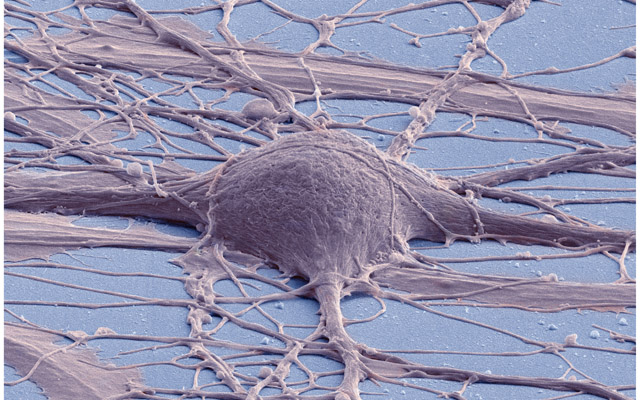
\includegraphics[scale=1.5]{../blog/images/2014_06_26_human_ipsc_derived_neuron_deerinck}
    \caption{Human neuron. Source: New Reprogramming Method Makes Better Stem Cells
      \url{http://ucsdnews.ucsd.edu/pressrelease/new_reprogramming_method_makes_better_stem_cells}.}
    \label{fig:3d_neuron}
\end{figure}

\end{frame}

\begin{frame}
\frametitle{Microscopy and computational neuroscience}

\begin{itemize}
\item The data generated by the microscopes cannot be used
  directly.
\pause
\item One must first perform recognition of the objects in the
  micrographs. This is known as \emph{segmentation} and
  \emph{reconstruction}.
\pause
\item Until recently these tasks were performed manually. Experienced
  lab technicians would identify and measure all of the structures in
  the neuron. This is a very low resolution and high-error process.
\pause
\item Recently Machine Learning has been applied to the task with
  success.
\end{itemize}

\end{frame}

\begin{frame}
\frametitle{Microscopy and computational neuroscience}

Sample micrograph from a stack. Left-hand side shows the original
micrograph; right-hand side shows the result of processing it with
machine learning.

\begin{figure}[H]
    \centering
    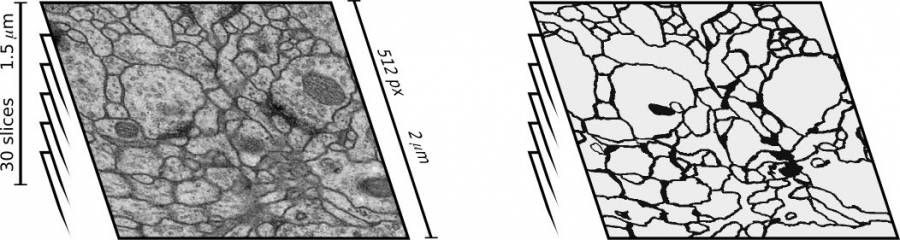
\includegraphics[scale=0.3]{../blog/images/biomed-neurons}
    \caption{Source: Deep Neural Networks Segment Neuronal Membranes in Electron Microscopy Images
      \url{http://papers.nips.cc/paper/4741-deep-neural-networks-segment-neuronal-membranes-in-electron-microscopy-images.pdf}.}
    \label{fig:stack}
\end{figure}

\end{frame}

\begin{frame}
\frametitle{Microscopy and computational neuroscience}

Reconstruction of 3D structures from a stack.

\begin{figure}[H]
    \centering
    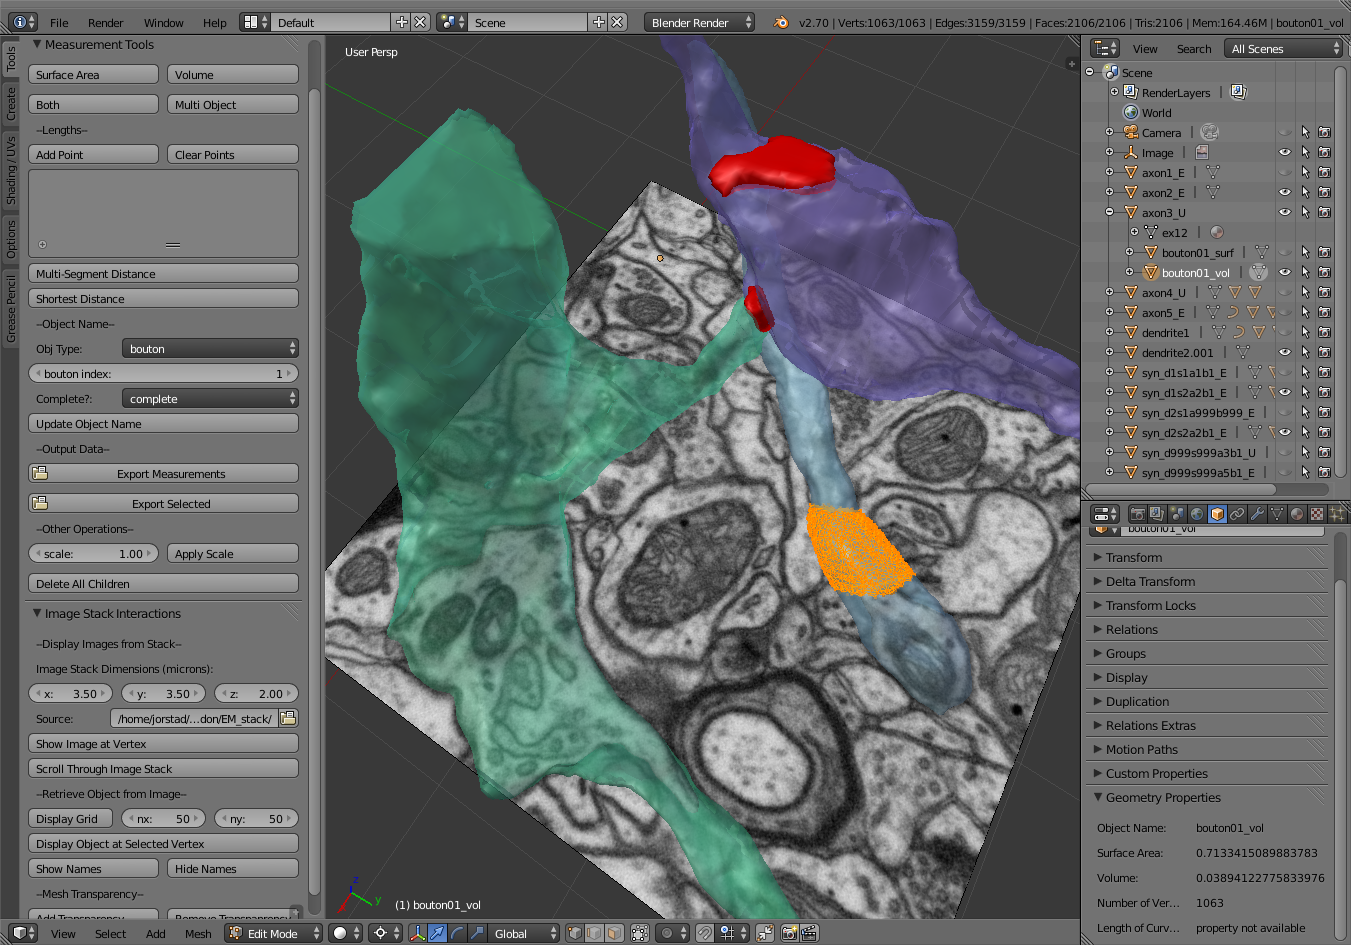
\includegraphics[scale=0.2]{../blog/images/NeuroMorph_screenshot.png}
    \caption{Source: Segmented anisotropic ssTEM dataset of neural tissue
      \url{http://figshare.com/articles/Segmented_anisotropic_ssTEM_dataset_of_neural_tissue/856713}.}
    \label{fig:3d_stack}
\end{figure}

\end{frame}

\begin{frame}
\frametitle{Microscopy and computational neuroscience}

Allen Brain Atlas user interface browsing a micrograph in a stack,
with corresponding reconstruction.

\begin{figure}[H]
    \centering
    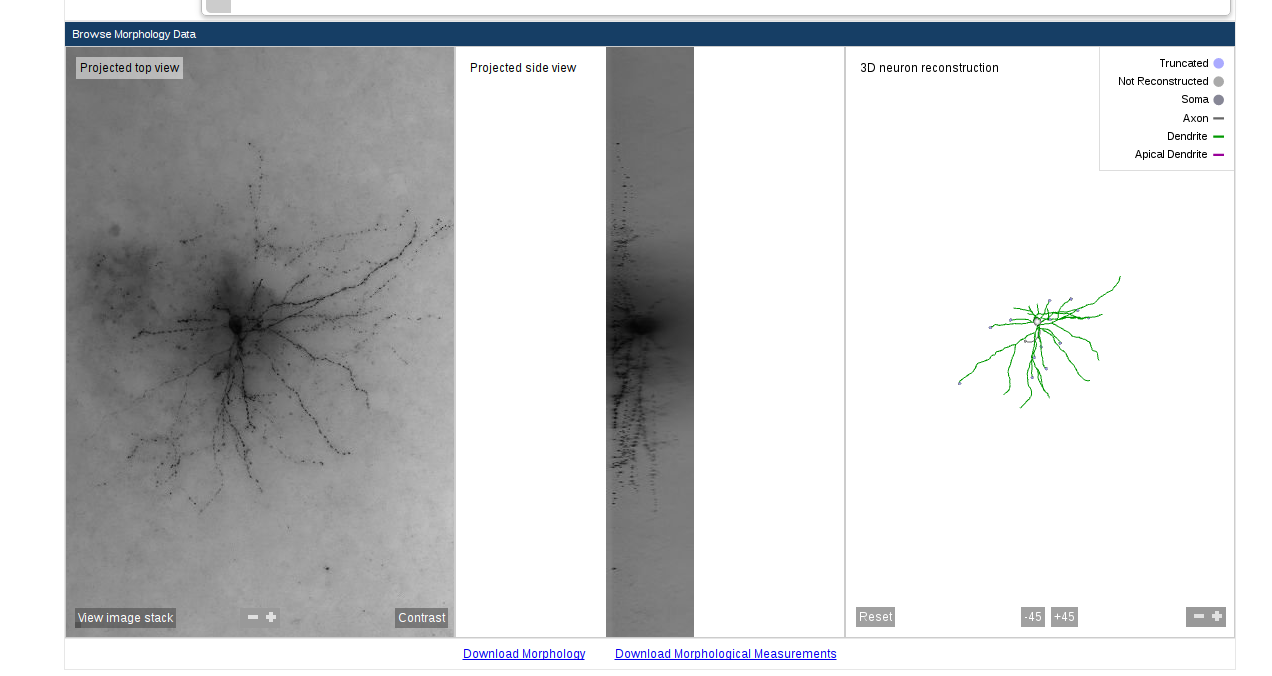
\includegraphics[scale=0.2]{../blog/images/allen_brain_atlas_primary_visual.png}
    \caption{Source: Allen Brain Atlas, Primary visual area, layer 5.
      \url{http://celltypes.brain-map.org/mouse/experiment/morphology/469610831}.}
    \label{fig:3d_stack}
\end{figure}

\end{frame}

\begin{frame}[fragile]
\frametitle{SWC}

\begin{itemize}

\item \emph{De facto} standard for storing morphology data.
\pause
\item As seen on Felix's presentation, the data is stored as a tree.
\pause
\item The internal format is a set of frusta (truncated cones),
  connected together in a parent and child relationship.
\pause
\item Powerful: morphometric work can be carried out from this simple
  tree representation, as per the functions provided by TREES and
  TREES2. Also useful for electrophysiology models, etc.
\pause
\end{itemize}

\begin{verbatim}
# id,type,x,y,z,r,pid
1 1 305.7912 312.7696 31.92 8.059 -1
2 2 307.4752 319.1016 31.9197 0.1144 1
3 2 307.7989 320.1896 31.8424 0.1731 2
5 2 309.0413 322.0349 31.7724 0.2652 4
...
\end{verbatim}
\end{frame}

\begin{frame}
\frametitle{SWC}

Example of measurements one may want to perform on a dendrite.

\begin{figure}[H]
    \centering
    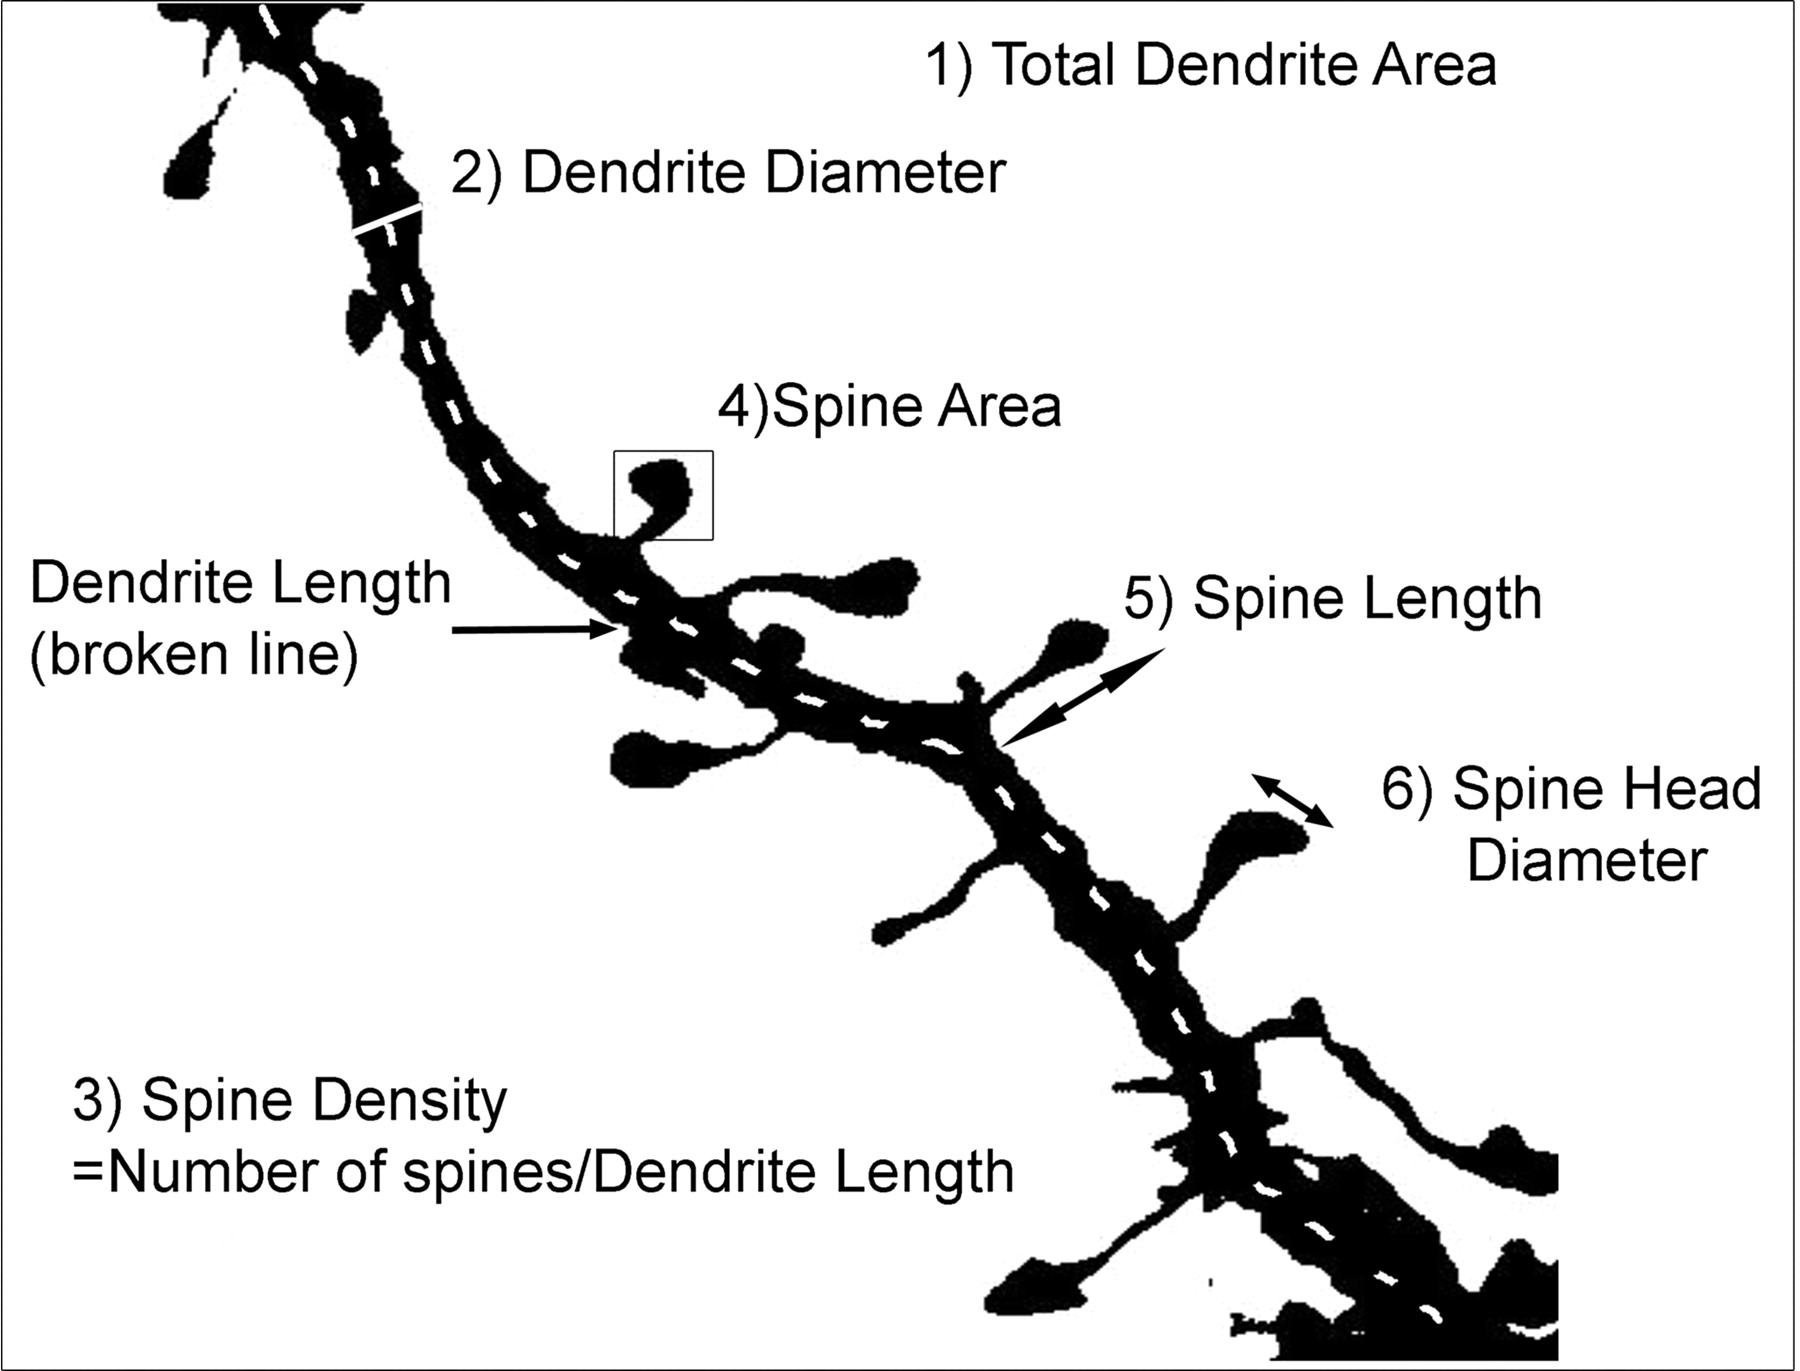
\includegraphics[scale=0.1]{../blog/images/F1_large}
    \caption{Source: Reversal of long-term dendritic spine alterations in Alzheimer disease models.
      \url{http://www.pnas.org/content/106/39/16877.abstract}.}
    \label{fig:morphometry}
\end{figure}

\end{frame}

\begin{frame}
\frametitle{SWC}

SWC is a good format which has withstood the test of time, but has
some important shortcomings.
\pause

\begin{itemize}
\item Microscopy has improved dramatically but the resolution SWC
  provides is frusta: all of the high-resolution detail is lost in the
  final representation.
\pause
\item Loss of detail is applicable to both soma and the dendrites: the
  soma is represented as a sphere or a similar solid; the dendrites
  may miss dendritic spines altogether or have very inaccurate
  representations.
\pause
\item SWC was designed in the nineties, where computer capacity (CPU,
  storage, network bandwidth, etc) was a fraction of what we have
  today. We no longer have the same constraints.
\pause
\item SWC provides limited extensibility for annotation and tagging
  of objects, including the reconstruction itself.
\pause
\end{itemize}

\end{frame}

\begin{frame}
\frametitle{SWC}

\begin{itemize}
\item For certain uses the loss of resolution may not have a
  significant impact: ``in electrophysiological models, the space
  constants are likely larger than geometric
  ambiguities''\cite{mcdougal2013water}.
\pause
\item In other cases it may be of great importance:
  \begin{itemize}
  \item Low-resolution is ``unsuitable for multi-scale models that
    also involve three-dimensional reaction-diffusion, as such models
    have smaller space constants.''\cite{mcdougal2013water}
  \pause
  \item Also, dendritic spine alterations are important in studies of
    Alzheimer's disease \cite{smith2009reversal}.
  \pause
  \end{itemize}
\item In addition, there may be new scientific questions that will
  only be posed when more accurate reconstructions are available.
\pause
\end{itemize}

\end{frame}

\begin{frame}
\frametitle{Polygon meshes}

Our approach is to use polygon meshes to provide more accurate
representations of neuronal morphologies.

\pause

\begin{itemize}
\item A polygon mesh is composed of large numbers of simple polygons
  such as triangles or quads. These are stitched together to represent
  a surface.
\pause
\item In an ideal world one would want to use volumetric meshes, which
  stitch together polyhedra to fill the represented volume. However,
  at present we are only looking at surface meshes.
\pause
\item We have additional requirements on surface meshes in order for
  them to be applicable to all use cases~--- morphometry,
  reaction-diffusion, electrophysiology, etc~--- which are not needed
  for other uses such as computer graphics/games.
\end{itemize}

\end{frame}

\begin{frame}
\frametitle{Polygon meshes}

Meshes must be completely manifold or watertight. This is a very
important requirement.
\pause

\begin{itemize}
\item Mathematical understanding: Non-manifolded edges are a
  problem. These are are parts of a model where the dots have not been
  connected to create a polygon. A line, or even a plane, does not have
  dimensions in three separate directions (x, y, z).
\pause
\item Intuitive understanding: if one were to fill in a physical
  representation of the model with water, would it have leaks.
\end{itemize}

\end{frame}

\begin{frame}
  \printbibliography
\end{frame}

\end{document}
